\documentclass[11pt,a4paper]{jsarticle}
\usepackage{amsmath,amssymb}
\usepackage{newtxtext,newtxmath}
\usepackage[dvipdfmx]{graphicx}
\usepackage{listings}
\lstset{%mactex
 language={C++},
 % backgroundcolor={\color[gray]{.95}},%
 tabsize=2, % tab space width
 showstringspaces=false, % don't mark spaces in strings
 basicstyle={\ttfamily},%
 %identifierstyle={\small},%
 commentstyle={\itshape},%
 keywordstyle={\bfseries},%
 %ndkeywordstyle={\small},%
 stringstyle={\ttfamily},
 %frame={tb},
 breaklines=true,
 columns=[l]{fullflexible},%
 % numbers=left,%
 % numberstyle={\small},%
 xrightmargin=0zw,%
 %xleftmargin=3zw,%
 stepnumber=1,
 numbersep=1zw,%
 lineskip=-0.5ex%
}
\lstset{%mactex
 language={R},
 % backgroundcolor={\color[gray]{.95}},%
 tabsize=2, % tab space width
 showstringspaces=false, % don't mark spaces in strings
 basicstyle={\ttfamily},%
 %identifierstyle={\small},%
 commentstyle={\itshape},%
 keywordstyle={\bfseries},%
 %ndkeywordstyle={\small},%
 stringstyle={\ttfamily},
 %frame={tb},
 breaklines=true,
 columns=[l]{fullflexible},%
 % numbers=left,%
 % numberstyle={\small},%
 xrightmargin=0zw,%
 %xleftmargin=3zw,%
 stepnumber=1,
 numbersep=1zw,%
 lineskip=-0.5ex%
}
\lstset{%mactex
 language={Python},
 % backgroundcolor={\color[gray]{.95}},%
 tabsize=2, % tab space width
 showstringspaces=false, % don't mark spaces in strings
 basicstyle={\ttfamily},%
 %identifierstyle={\small},%
 commentstyle={\itshape},%
 keywordstyle={\bfseries},%
 %ndkeywordstyle={\small},%
 stringstyle={\ttfamily},
 %frame={tb},
 breaklines=true,
 columns=[l]{fullflexible},%
 % numbers=left,%
 % numberstyle={\small},%
 xrightmargin=0zw,%
 %xleftmargin=3zw,%
 stepnumber=1,
 numbersep=1zw,%1
 lineskip=-0.5ex%
}
\begin{document}

\title{ニューラルネットワーク \\
PRML輪読会 第1回資料}
\author{西本 洋紀 \\
        教養学部学際科学科B群 2年
        }
\date{\today}
\maketitle
%-----------------------------------------------------------------------------------------------------
\section*{はじめに}
本稿は平成31年2月10日開催のPRML輪読会第1回資料として作成した. \\
筆者の理解では, 第5章は, 大きく5つの部分に分けられていると考える. \\
まずはじめに、ニューラルネットワークの中でも特にフィードフォワードネットワークに限定して話を進める. 線形回帰/分類モデルとの比較において、フィードフォワードネットワークの関数の形を見る.\\
次に、ネットワークパラメータを決定する問題を扱う. 最尤推定の枠組みからこの問題を議論する.これには、非線形化最適化問題をどう解くかという問題も含まれる. その後「誤差逆伝播」について確認し、この方法がヤコビ行列、ヘッセ行列に対して拡張されることを見る.\\
次に、ニューラルネットワークの正規化への様々なアプローチと互いの関係について確認する.\\
ここまでニューラルネットワークの中でも特にフィードフォワードネットワークに限定した話であったが、次にフィードフォワードネットワーク以外のニューラルネットワークに話題を転じる.特に混合密度ネットワークという、条件付き確率分布をモデル化する枠組みについて扱う.\\
最後に、ベイズ理論の立場からニューラルネットワークについて議論する.
\subsection*{用語についての確認}
本題に入るまでに、本稿で用いられる用語の中で注意が必要ないくつかのものについて、意味を確認しておく.
\begin{itemize}
  \item ニューラルネットワーク\\
  本稿の表題となっているこの語は、生体システムにおける情報システムを数学的に表現しようという試みにその語源がある.しかし、本稿では、「パターン認識という実際的な応用の観点からは、生物学的な現実性などは全くの不要な制約である」という、PRML著者の見解に倣い、統計的パターン認識のための効率的なモデルとしてのニューラルネットワークを扱うこととする.
  \item 多層パーセプトロン(Multilayer perceptron)
  後述するフィードフォワードネットワークの別名としても知られ、実用面で最も高く評価されている特別なニューラルネットワークである.本稿の前半では、ニューラルネットワークの中で特にこのネットーワークに限定して説明を進める.しかし、多層パーセプトロンは実際は(不連続な非線形性をもつ)複数のパーセプトロンではなく、(連続的な非線形性を持つ)ロジスティック回帰モデルを多層にしたものなので、この呼び方は本当はあまり適切でない.以降、本稿では、フィードフォワードネットワークに呼び名を統一して説明を進めることとする.

\end{itemize}
\section{フィードフォワードネットワーク関数}
この章では, 3章、4章で議論した線形回帰/分類モデルとの違いに着目しながら、フィードフォワードネットワークの関数の形を
見ることとする.まず、3章、4章で議論した線形回帰/分類モデルは下のように定式化されるのであった.\\
\begin{equation}
  y(\textbf{x}, \textbf{y}) = f(\textbf{w}^T \phi(\textbf{x}))
\end{equation}
ここで、$\phi(\textbf{x})$は基底関数である. 回帰問題ではfは恒等関数、分類問題ではfは非線形活性化関数である. 学習の際は、固定された基底関数$\phi(\textbf{x})$に対し、最適な$\textbf{w}$(の確率分布)を決める問題を解くのであった.\\これらのモデルは、解析や計算においては有用な性質を持つが、次元の呪いのために実際的な応用可能性は限られる. このようなモデルを大規模な問題に適用するためには基底関数をデータに適応させる必要があるが、その1つのアプローチとして、基底関数に対してパラメトリック形を用い、そのパラメータ値を訓練中に適応させる、フィードフォワードネットワークが知られている. これは次のように定式化される. ただし、$f$は出力層の関数に相当し、回帰問題の時は恒等関数、2クラス分類の時はロジスティック関数、他クラス分類の時はSoftmax関数を用いる. 問題の形によって出力層の関数が変化するという点は、後で本稿2節で議論する.\\
\begin{equation}
  y(\textbf{x}, \textbf{y}) = f(\sum_{j=0}^M w_{kj} ^{(2)} h(\sum_{i=0}^D w_{ji}^{(1)}x_i))\\
                            = f(\sum_{j=0}^M w_{kj} ^{(2)} \phi_j(\textbf{x}))
\end{equation}
この式を見ると、基底関数に対してパラメトリック形が用いられている様子がよくわかるのではないだろうか. 実際、学習の際は、基底関数の線型結合のパラメータのみならず、基底関数を決定するパラメータも決定する問題を解くことになる. \\
下図は、上式(2)に相当する2層ニューラルネットワークの図である. 入力変数、隠れ変数、出力変数はノードとして表され、重みパラメータは、$入力変数x_0と隠れ変数z_0を追加し、そこからのリンクの重みとして表されている.この図において、基底関数の線型結合のパラメータは、$出力層と隠れユニットをつなぐリンクの重みづけに相当し、基底関数を決定するパラメータは、隠れユニットと入力層をつなぐリンクの重みづけに相当している.上式(2)に従ってyを評価する過程は、ネットワークの情報の\textbf{順伝播}と解釈することができる.\\
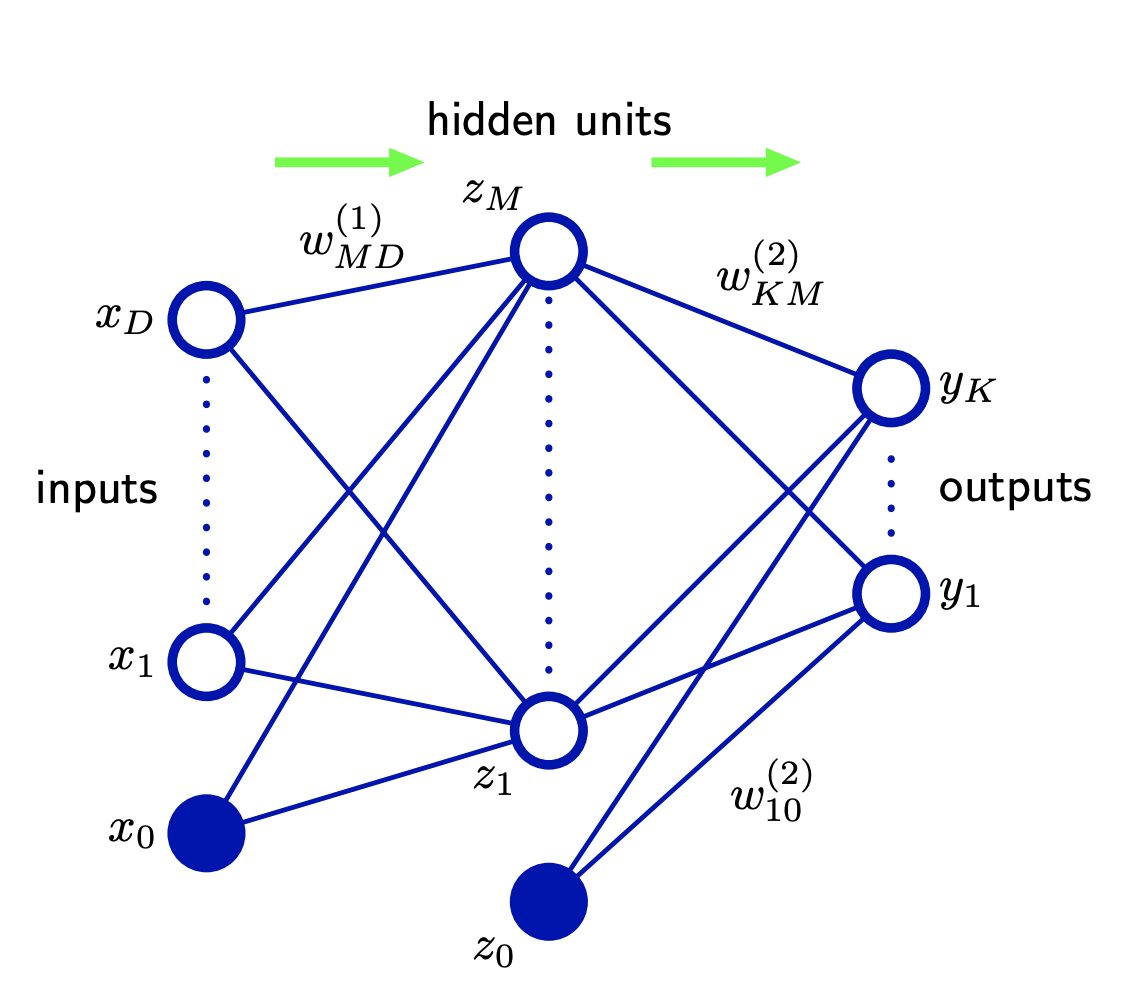
\includegraphics[scale=0.4]{neuralnet.png}
\subsection*{ネットワーク構造の一般化}
上図に示すネットワーク構造はごく普通に使われるものであるが、これは簡単に拡張される。例えば、\\
\begin{equation}
  a_k = \sum_{j=1}^M w_{kj}^{(2)} z_j + w_{k0}^{(2)} ~ (k = 1,...,K)
\end{equation}
のように重み付き和を計算し、それを非線形活性化関数を用いて変換するようなユニットからなる層を複数追加することなどが可能である.\\もう1つのネットワークの構造の一般化は、層を飛び越えた結合である(下図参照).下図ではわかりやすさのため省略されているが、隠れユニットと出力層はそれぞれバイアスパラメータを持つことに注意が必要である.ネットワーク図は数学的な関数と直接対応しているので、より複雑なネットワークを考えることで、より一般的な写像に発展させることができる.しかしながら、出力が入力の決定論的な関数であることを保証するために、有向閉路を持たないフィードフォワード構造である必要がある.\\
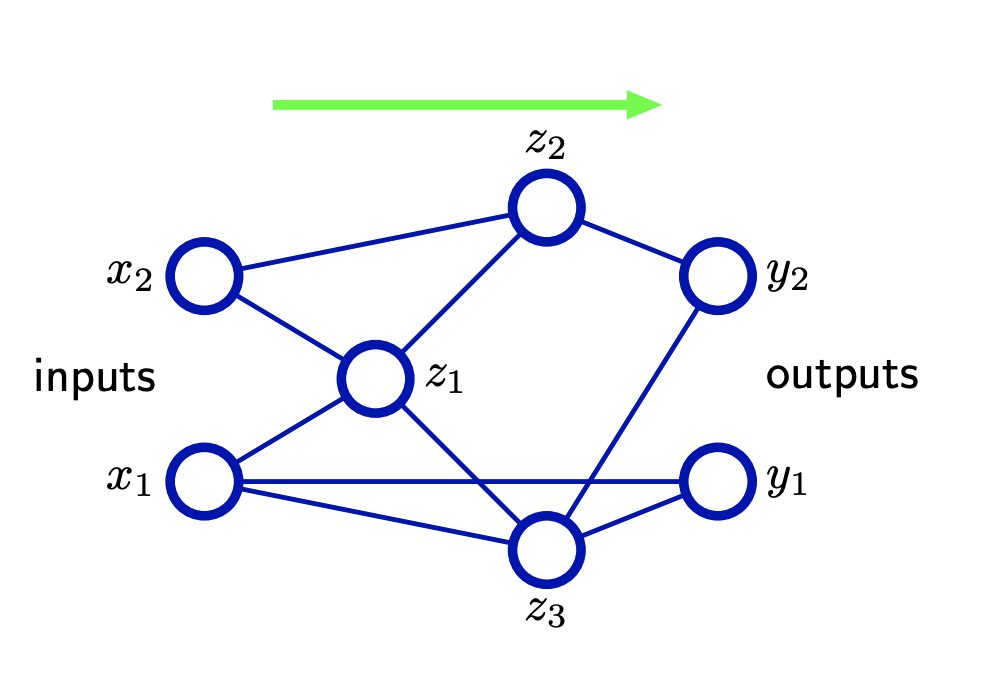
\includegraphics[scale=0.4]{jump.png}
\\このようなネットワークの隠れユニットあるいは出力層は\\
\begin{equation}
z_k = h(\sum_{j} q_{kj} z_j)
\end{equation}
で与えられる関数を計算する. ここで、和はユニットkへ接続を持つ全てのユニットに対してとる(バイアスパラメータも含む).与えられたネットワークの入力に対して、式(4)を順番に当てはめることで、ネットワークの活性を出力層を含めて評価することができる.\\
\subsection{フィードフォワードネットワークの優れた関数近似特性を示す例}
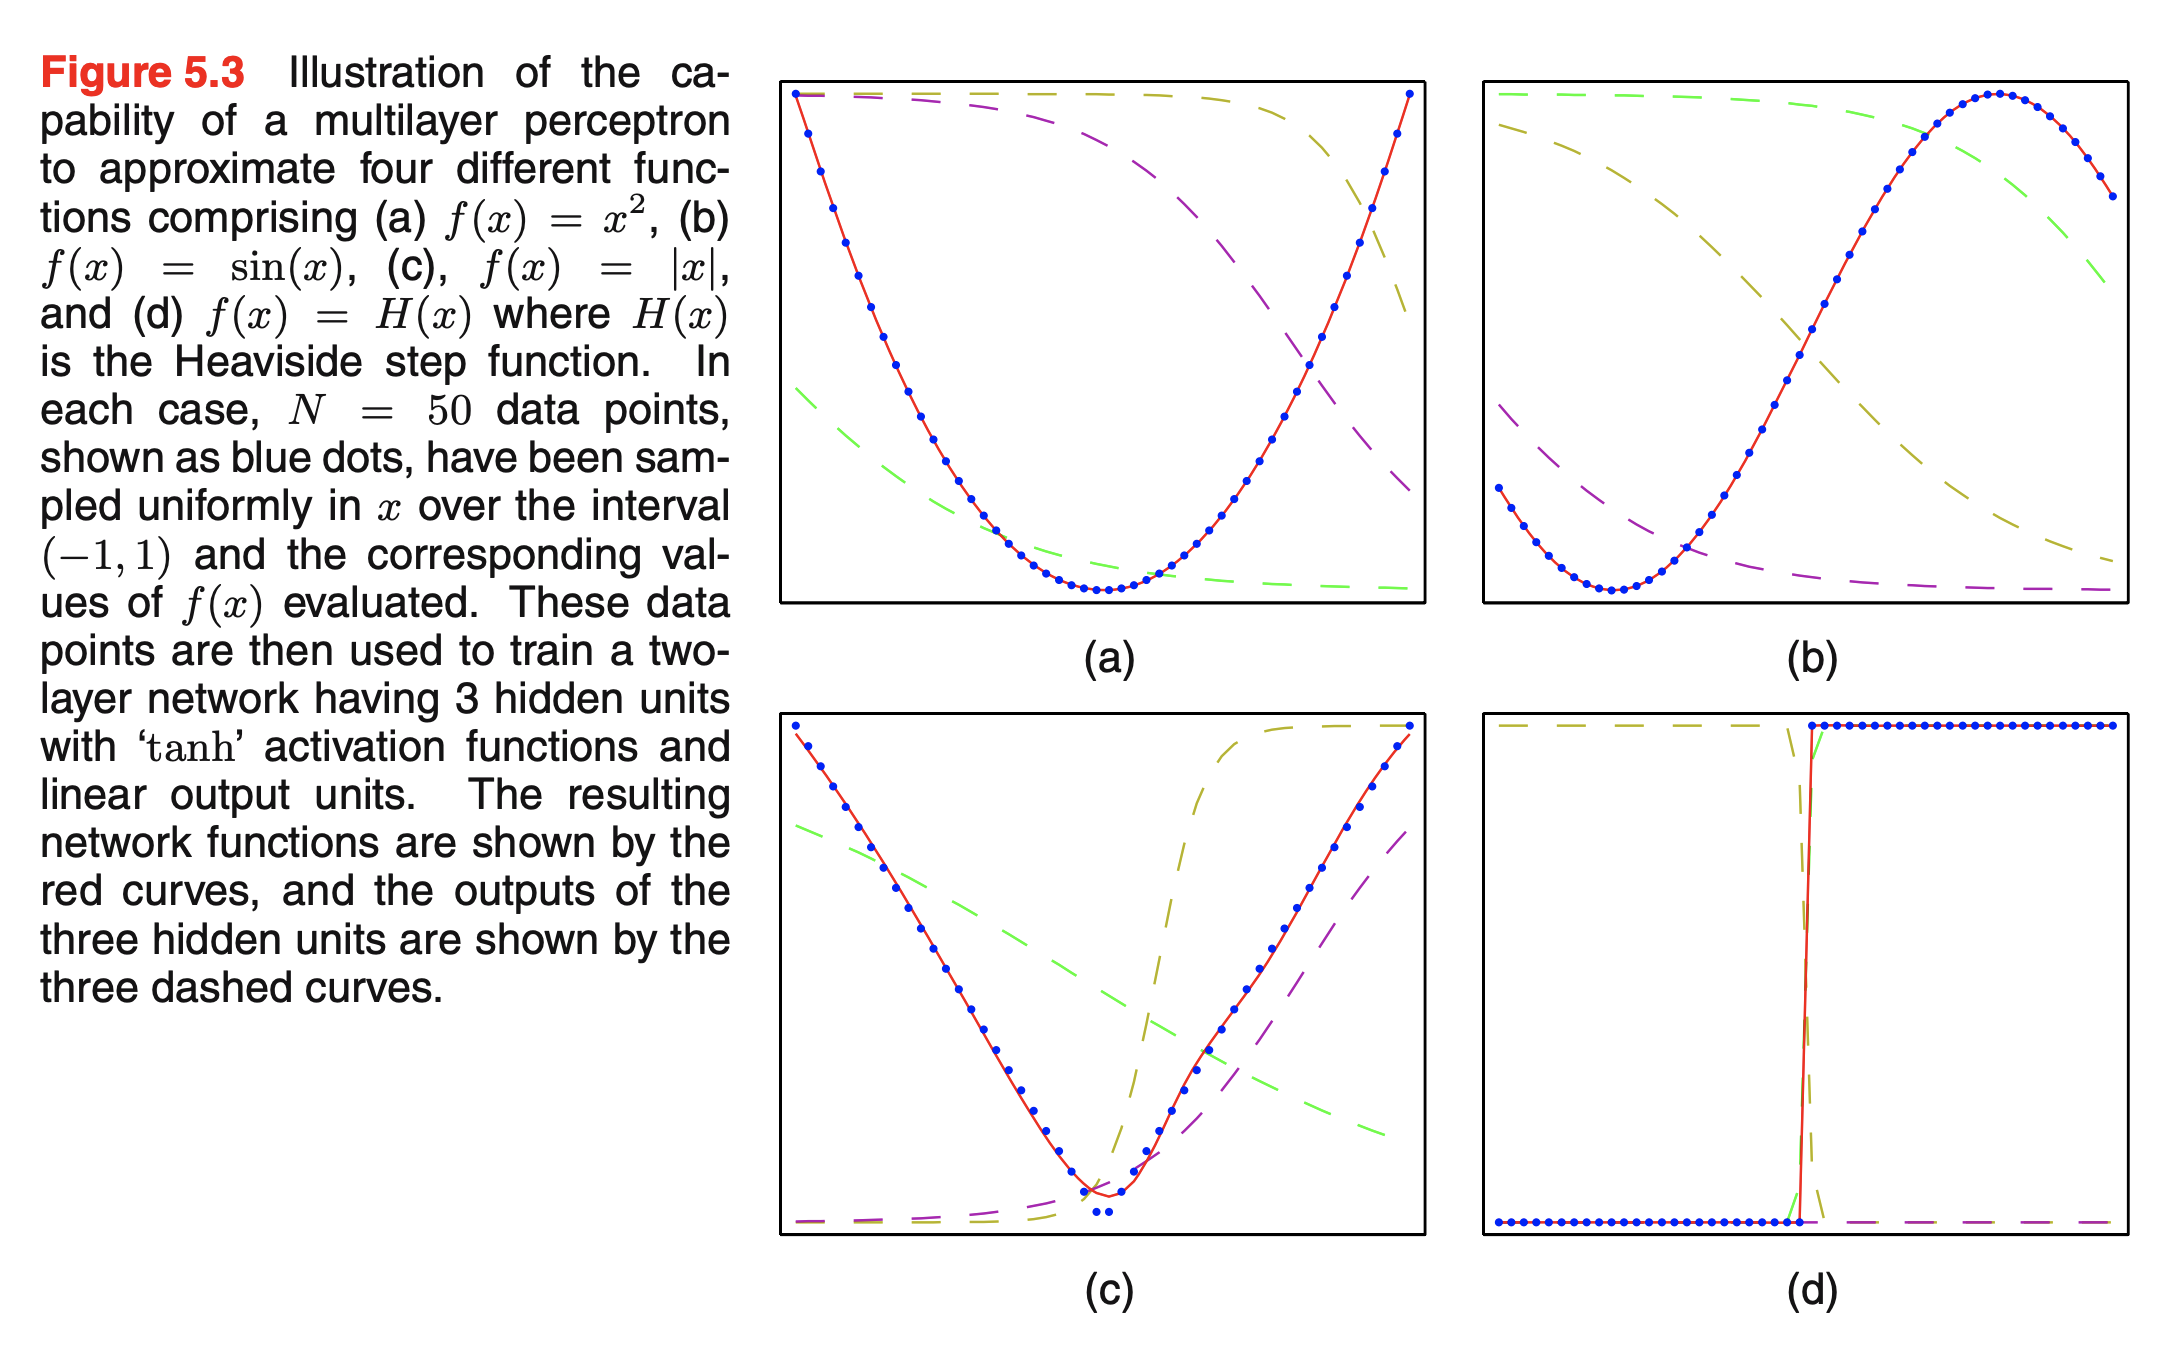
\includegraphics[scale=0.4]{example.png}
\newpage
\section{ネットワーク訓練}
ここまで、ニューラルネットワークを入力変数$\textbf{x}から出力変数のベクトル\textbf{y}$へのパラメトリックな非線形関数の一般的なクラスとしてみてきた. 次に、隠れユニットのパラメータや、出力層のパラメータの最適化をどのように行うかについて議論する.
\subsection{最尤推定}
\subsection*{ネットワーク出力の確率的な解釈}
最尤推定によるネットワークパラメータの最適化を考える前に、ネットワーク出力の確率的な解釈を考える. これにより、出力層の非線形活性化関数の選択と誤差関数の選択に、明確な誤差関数の選択に、明確な理由づけができるようになる.
\begin{itemize}
  \item 回帰問題\\
  任意の実数値を取れる1つの目標変数tを考える. tはxに依存する平均を持つガウス分布に従うことにする. ただしその平均は
  \begin{equation}
    p(t|\textbf{x}, \textbf{w})  = N(t|y(\textbf{x}, \textbf{w}) ,\beta^{-1})
  \end{equation}
  のように、ニューラルネットワークの出力で与えられる.式(5)で与えられる条件付き分布に対しては、出力層の活性化関数は恒等写像をとれば十分である. というのは、そのようなネットワークで任意の$\textbf{x}からyへの連続関数を近似できるからである.N個の 独立同分布に従う観測値\textbf{X} =\{x_1,x_2,...,x_N\}とそれぞれに対応する目標値\textbf{t}=\{t_1,t_2,...,t_N\}$からなるデータ集合が与えられた時、尤度関数は
  \begin{equation}
    p(\textbf{y}|\textbf{X},\textbf{w}, \beta)  = \prod_{n=1}^{N} p(t_n | \textbf{x}_n, \textbf{w}, \beta)
  \end{equation}
  と表される.負の対数を取ると誤差関数
  \begin{equation}
    \frac{\beta}{2} \sum_{n=1}^{N} \{y(\textbf{x}_n)-t_n \}^2 - \frac{N}{2} ln \beta + \frac{N}{2} ln(2 \pi )
  \end{equation}
  が得られ、これを用いて$パラメータ\textbf{w}および\beta$を学習することができる. \textbf{w}について最大化する. 尤度関数を最大化することは、加法および乗法定理の違いを無視すると
  \begin{equation}
    E(\textbf{w})=\frac{1}{2}\sum_{n=1}^{N} \{y(\textbf{x}_n, \textbf{w} - t_n)^2
  \end{equation}
  で与えられる二乗和誤差関数の最小化と等価である.$E(\textbf{w})を最小化する\textbf{w}は最尤推定の会に相当するので、\textbf{w}_{ML}と表すことにする.現実に得られるのは尤度の極大点(誤差関数の極小点に相当)である.このことは次節で議論する.$
  $\textbf{w}_{ML}が求まれば、\beta$の値は負の対数尤度を最小化することで得られ、
  \begin{equation}
    \frac{1}{\beta_{ML}} = \frac{1}{N} \sum_{n=1}^{N} \{y(\textbf{x}_n, \textbf{w}_{ML}) - t_n \} ^2
  \end{equation}
  と与えられる.\\
  回帰関数の場合、ネットワークは恒等写像の出力活性化関数$y_k = a_k$を持つとみなせ、それに対応する二乗和誤差関数には\\
  \begin{equation}
    \frac{\partial E}{\partial a_k} = y_k - t_k
  \end{equation}
  という性質がある. これは誤差逆伝播を議論するときに利用される.
  \item 2クラス分類問題
  \item 多クラス分類問題
  \item まとめ
  出力層の活性化関数および対応する誤差関数は、解くべき問題の方によって自然に選択される.回帰問題においては、線形出力関数および二乗和誤差を使い、2クラス分類問題では、ロジスティックシグモイド関数および交差エントロピー誤差関数を使い、そして他クラス分類問題においては、ソフトマックス関数およびそれに対応する他クラス交差エントロピー誤差関数を使う。2クラス分類問題においては、単一のロジスティックシグモイド関数を使うこともできるし、ソフトマックス活性化関数を持つ2出力のネットワークを使うこともできる.
\end{itemize}
\subsection*{パラメータ最適化}
\subsection*{局所2次近似}
\subsection*{誤差逆伝播}
\subsection*{ヤコビ行列}
\subsection*{ヘッセ行列}
\section{ニューラルネットワークの正則化}
\section{混合密度ネットワーク}
\section{ベイズニューラルネットワーク}
\end{document}
